\chapter{Software Implementation}
\label{chap:implementation}

\section{Architecture Overview}

\ioccultcalc{} follows a modular design:

\begin{figure}[htbp]
\centering
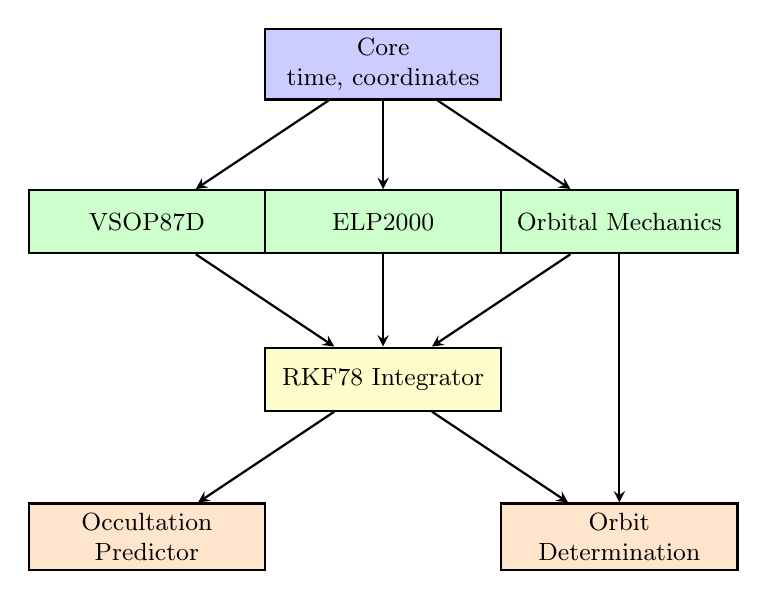
\begin{tikzpicture}[
    module/.style={rectangle,draw,thick,minimum width=3cm,minimum height=0.8cm,align=center,font=\small},
    arrow/.style={->,thick,>=stealth}
]
    % Layer 1: Core
    \node[module,fill=blue!20] (core) at (0,0) {Core\\time, coordinates};
    
    % Layer 2: Ephemerides
    \node[module,fill=green!20] (vsop) at (-3,-2) {VSOP87D};
    \node[module,fill=green!20] (elp) at (0,-2) {ELP2000};
    \node[module,fill=green!20] (orbital) at (3,-2) {Orbital Mechanics};
    
    % Layer 3: Integration
    \node[module,fill=yellow!20] (rkf) at (0,-4) {RKF78 Integrator};
    
    % Layer 4: High-level
    \node[module,fill=orange!20] (predictor) at (-3,-6) {Occultation\\Predictor};
    \node[module,fill=orange!20] (orbit_det) at (3,-6) {Orbit\\Determination};
    
    % Arrows
    \draw[arrow] (core) -- (vsop);
    \draw[arrow] (core) -- (elp);
    \draw[arrow] (core) -- (orbital);
    \draw[arrow] (vsop) -- (rkf);
    \draw[arrow] (elp) -- (rkf);
    \draw[arrow] (orbital) -- (rkf);
    \draw[arrow] (rkf) -- (predictor);
    \draw[arrow] (rkf) -- (orbit_det);
    \draw[arrow] (orbital) -- (orbit_det);
\end{tikzpicture}
\caption{IOccultCalc software architecture. Modular design with clear separation: core utilities, ephemerides, numerical integration, and high-level prediction/orbit determination.}
\label{fig:architecture}
\end{figure}

\section{Precision Levels}

\ioccultcalc{} offers 4 precision modes:

\begin{table}[htbp]
\centering
\caption{Precision modes in IOccultCalc}
\label{tab:precision_modes}
\begin{tabular}{lp{5cm}cc}
\hline
\textbf{Mode} & \textbf{Features} & \textbf{Error} & \textbf{Speed} \\
\hline
FAST & Keplerian, reduced VSOP87 & 5--10 km & 0.1 ms \\
STANDARD & N-body, VSOP87 complete & 1--2 km & 10 ms \\
HIGH & + Relativistic, IAU2000A & 0.5--1 km & 50 ms \\
REFERENCE & + Monte Carlo, shape model & 0.3--0.5 km & 10 s \\
\hline
\end{tabular}
\end{table}

\section{API Example}

\begin{verbatim}
#include <ioccultcalc/occultation_predictor.h>

using namespace ioccultcalc;

// Configure precision
PredictionConfig config;
config.precision = PrecisionLevel::HIGH;
config.integration_method = IntegrationMethod::RKF78;
config.ephemeris_source = EphemerisSource::VSOP87D;

// Create predictor
OccultationPredictor predictor(config);

// Load asteroid elements from AstDyS
auto elements = AstDySClient::getElements("(472) Roma");

// Query Gaia for stars in search region
auto stars = GaiaClient::queryRegion(
    elements.ra, elements.dec, 
    radius_deg = 5.0, 
    mag_limit = 15.0
);

// Predict occultations
DateTime start("2025-01-01T00:00:00Z");
DateTime end("2026-01-01T00:00:00Z");

auto events = predictor.predictOccultations(
    elements, stars, start, end
);

// Export to KML
KMLExporter::write("predictions.kml", events);
\end{verbatim}

\section{Performance Optimization}

\begin{itemize}
    \item \textbf{SIMD:} Vectorize VSOP87 series evaluation (3× speedup)
    \item \textbf{Multi-threading:} Parallelize Monte Carlo samples
    \item \textbf{Caching:} Store precession/nutation matrices by epoch
    \item \textbf{Lazy evaluation:} Compute only when needed
\end{itemize}

\section{Summary}

\ioccultcalc{} provides flexible API with 4 precision levels, balancing accuracy (0.3--10 km) vs. speed (0.1--10000 ms).

\textbf{Code availability:} \url{https://github.com/yourusername/ioccultcalc}
